\chapter{Modelo de Seguridad de iOS}
iOS es un sistema operativo para dispositivos móviles de la multinacional Apple Inc. diseñado para ser
seguro \cite{asg}. Cada dispositivo combina hardware, software y servicios, diseñados para trabajar
conjuntamente para proveer seguridad y al mismo tiempo, que sea transparente para el
usuario.\\
Características como el cifrado del sistema de archivos, asegurar un arranque seguro, proveer un repositorio de contraseñas seguro, vienen habilitadas por defecto. Como se puede observar en la Figura \ref{fig:ch02:security-architecture}, la seguridad se extiende más allá del dispositivo, generando un ecosistema seguro.\\
\begin{figure}[hbtp]
    \centering
    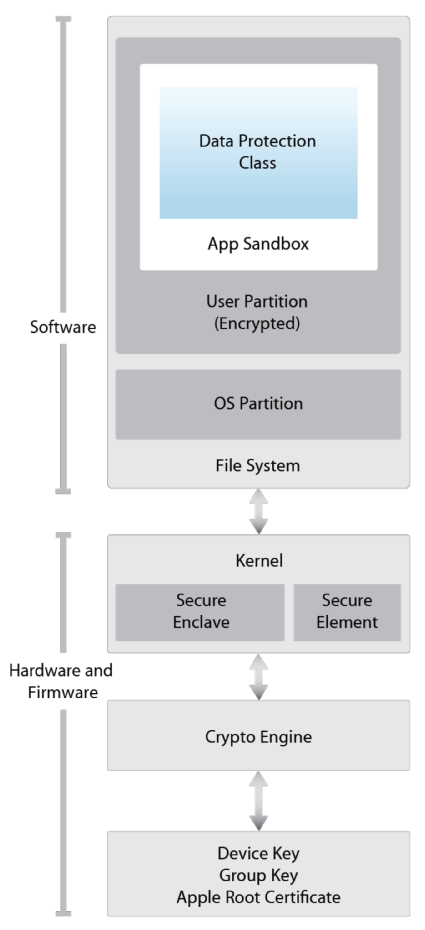
\includegraphics[width=0.3295\linewidth]{chapter2/ios_security_architecture}
    \caption{Modelo de seguridad de iOS \cite{asg}.} 
    \label{fig:ch02:security-architecture}
\end{figure}
\newpage
A lo largo de este capítulo se realizara una descripción de los principales aspectos del modelo de seguridad de iOS, basándose en la versión 9.3, lanzada en 2015.
\section{Protección de los datos} \label{fig:ch02:data-protection}
iOS tiene una protección especial para los archivos y los datos personales, la cual sigue intacta inclusive si algunas otras partes del sistema de seguridad fueron comprometidas \cite{asg}. La protección de los datos es implementada construyendo varias claves criptográficas y generando con ellas una jerarquía.\\
El dispositivo móvil provee un componente de \textit{hardware} llamado \textit{Secure Enclave}. Es un coprocesador con memoria cifrada e incluye generación de números aleatorios por hardware. Tiene tres responsabilidades principales:
\begin{itemize}
    \item proveer las operaciones de cifrado para la manipulación de la Clave de los Datos\footnote{Traducción propuesta para el término \textit{Data Protection Key}.};
    \item mantener la integridad de dichos datos inclusive si \textit{kernel} haya sido comprometido;
    \item es el responsable de procesar los datos provenientes del \textit{Touch ID}\footnote{\textit{Touch ID} es el sistema de detección de huellas digitales que hace posible un acceso seguro, más rápido y sencillo al dispositivo.}, determinando si se desbloquea el dispositivo.
\end{itemize}
En los procesadores A9 o posteriores de la serie A, el chip genera de forma segura el identificador único UID\footnote{\textit{Unique ID}, por sus siglas en inglés.}. Esta clave fue creada en el momento de fabricación y que no es conocida por Apple ni por ningún otro componente del dispositivo. La misma es utilizada para generar una clave efímera cada vez que se prende el dispositivo, la cual se utiliza para cifrar la memoria del \textit{Secure Enclave} y los datos del sistema de archivos.\\
El UID permite vincular los datos a un dispositivo determinado mediante cifrado. Por ejemplo, la jerarquía de claves que protege el sistema de archivos incluye el UID, de modo que si los chips de memoria se trasladan físicamente de un dispositivo a otro, no será posible acceder a los archivos.
\section{Código de desbloqueo}
Al configurar el código de desbloqueo para un dispositivo, el usuario activa la protección de datos automáticamente. El sistema admite códigos alfanuméricos de cuatro dígitos, de seis dígitos y de longitud arbitraria, salvo que el dispositivo tenga un lector de huellas; en ese último caso deberá contar con al menos seis dígitos.\\
Además de desbloquear el dispositivo, el código provee entropía a ciertas claves de cifrado del sistema. El hecho de que esté muy ligado con el UID, añade una seguridad extra: no se puede intentar quebrar dicho código fuera del dispositivo. Es por ello que cuanto más seguro sea el código de desbloqueo, más segura será la clave de cifrado.\\
A fin de desalentar los posibles ataques de fuerza bruta, se generan retardos cada vez mayores tras la introducción de un código inválido en la pantalla de bloqueo. Los retardos están calibrados suponiendo que la frecuencia entre un ataque y otro es de 80 milisegundos \cite{asg}. En dispositivos que cuentan con un \textit{Secure Enclave}, los retardos se aplican mediante dicho componente. Si el dispositivo se reinicia durante un tiempo de demora, la demora aún se aplica, con el temporizador empezando de nuevo para el periodo actual.
\section{Seguridad en las aplicaciones}
\subsection{Entorno seguro}
Las aplicaciones son un punto crítico en la seguridad de un dispositivo móvil. Es por ello que iOS provee varias capas de seguridad para las aplicaciones, asegurando que una aplicación esté certificada y verificada antes de estar disponibles en la tienda \cite{asg}.\\
\begin{figure}[hbtp]
	\centering
	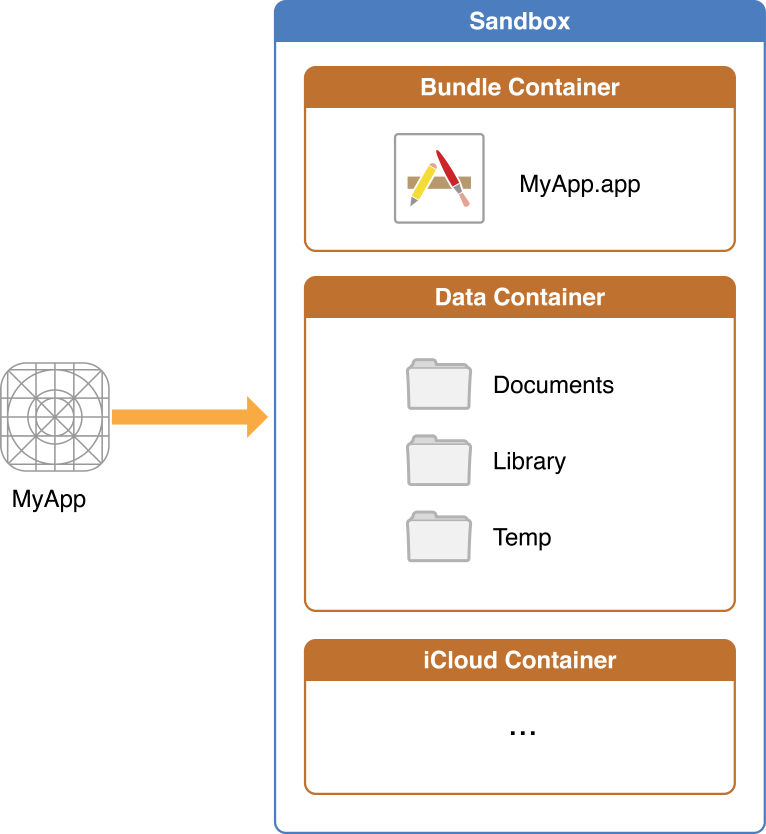
\includegraphics[width=.5\linewidth]{chapter2/ios_about_sandboxing}
    \caption{Entorno aislado de una aplicación en iOS \cite{iosdl}} 
    \label{fig:ch02:sandboxing}
\end{figure}
Cada aplicación instalada por el usuario se ejecuta en un \emph{entorno aislado}\footnote{Traducción propuesta para el término \textit{sandbox}.}. Como consecuencia de esto, tiene denegado el acceso de archivos guardados por otra aplicación y no puede realizar cambios en el dispositivo. Si una aplicación requiere acceder a información que no es suya, lo puede hacer únicamente usando servicios de iOS. Lo mismo sucede si quiere ejecutar procesos en segundo plano. En la Figura \ref{fig:ch02:sandboxing} se puede observar lo mencionado anteriormente: cada aplicación tiene su directorio \textit{Home} para sus archivos, el cual es otorgado aleatoriamente al momento de la instalación.\\
El entorno seguro de una aplicación comienza desde el momento de su desarrollo. Los IDE de iOS construyen las aplicaciones utilizando las técnica ASRL\footnote{\textit{Address Space Layout Randomization} es una técnica de seguridad informática involucrada en la prevención contra ataques de desbordamiento de \textit{buffer}.}. Por ejemplo, Xcode compila automáticamente con ASLR activada. De esta forma, se asegura que todas las regiones de memoria son aleatorias al momento de ejecución \cite{asg}, reduciendo la probabilidad de muchos \textit{exploits} sofisticados.
\subsection{Controles de privacidad}
iOS ayuda a evitar que las aplicaciones accedan a la información personal de un usuario sin permiso. Es por ello que, el acceso a ciertos recursos, necesita autorización explícita del usuario. Las aplicaciones pueden solicitar un permiso solamente mientras se esté ejecutando. A su vez, los usuarios pueden optar por no permitir este acceso, y pueden cambiar su elección en cualquier momento. Cabe aclarar que una aplicación puede utilizar un recurso sólo si se le ha dado permiso.\\
Los permisos restringen el acceso a:
\begin{multicols}{2}
    \begin{itemize}
        \item Servicios de Localización
        \item Contactos
        \item Calendarios
        \item Recordatorios
        \item Fotos
        \item Compartir Bluetooth
        \item Micrófono
        \item Cámara
        \item Salud
        \item \textit{HomeKit}
        \item Redes Sociales
    \end{itemize} 
\end{multicols}
Finalmente, los usuarios pueden ver qué aplicaciones han permitido acceder a cierta información, así como otorgar o revocar cualquier acceso futuro. Dicha información se encuentra en la configuración de privacidad (\texttt{Ajustes/Privacidad}), como se observa en la Figura \ref{fig:ch02:permissions-capture}.\\
\begin{figure}[hbtp]
    \centering
    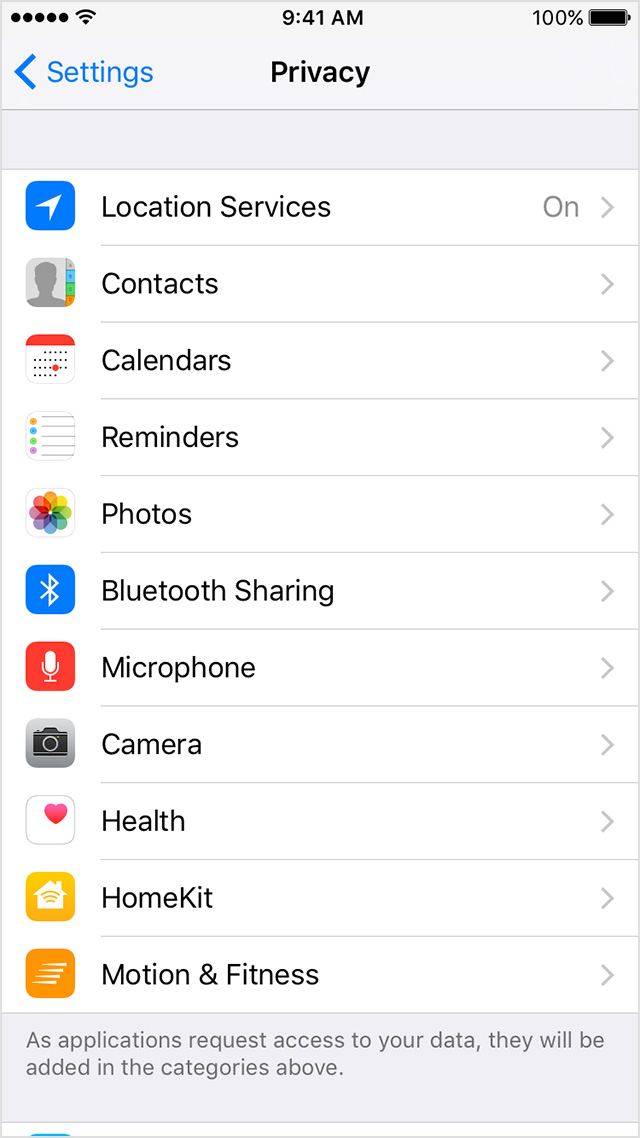
\includegraphics[width=.3\linewidth]{chapter2/settings-privacy}
    \caption{Control de privacidad de iOS 9.}
	\label{fig:ch02:permissions-capture}
\end{figure}
